\scanpage{49}\mspage{48}
\deleted{$G$ such that $F_{X'}\subset G'$ i.e. $X'\in G'$. This subdivision is induced by subdivision $G'\cup(F\setminus G)$, which is disjoint, and since}
\[
\deleted{X'\in G'}
\]
\deleted{\unsure{Suppose} \unsure{a|a}}
\figure{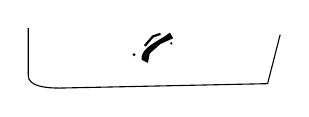
\begin{tikzpicture}[x=1cm,y=1cm,scale=.8]
\draw (0,.9)--(0,.15)..controls(0,-.03)and(.3,-.05)..(.5,-.05)--(3.8,.02)--(4,.8);
\fill (1.8,.4)..controls(1.78,.55)and(1.96,.65)..(2.15,.76)--(2.25,.83)--(2.3,.74)--(2.1,.65)--(1.93,.5)--(1.9,.35)--cycle;
\draw[line width=.8pt] (1.85,.62)--(1.98,.77)--(2.1,.81);
\fill(1.68,.48)circle(.025);\fill(2.27,.66)circle(.02);
\end{tikzpicture}}

\deleted{\uline{Proposition}}\inserted{Corollary 3} Let $\deleted{F}G,F$ be two figures. For $\deleted{F}G\subset F$\inserted{ (i.e. $G$ subfigure of $F$)}, it is necessary and sufficient that $\deleted{F}G$ \uline{compatible} with $F$ (i.e. $\deleted{\unsure{G|F}}F\cup\deleted{F}G$ a figure, say $\deleted{\unsure{F|G}}H$) and $\deleted{F}G\ll F$, i.e $G\subset\deleted{G'}F'$, $\deleted{\unsure{G|F}}F'$ subdivision of $F$.

Indeed, by \deleted{\unsure{Cont|Cond|C}} C 4, \deleted{since}
\diagram{\begin{tikzcd}[ampersand replacement=\&,row sep=.15em,column sep=.25em]
F \& \subset \& H=F\cup G \\
F'\arrow[u,Rightarrow,"\text{subdivision}"] \& {} \& {}\\
\tikz[baseline=-.5ex]\node[rotate=90,inner sep=0pt] {$\subset$}; \& {} \& {}\\
\deleted{\unsure{F|G}}G \& {} \& {}
\end{tikzcd}}
% The following calculation is written immediately to the right of the diagram.
\[
G\subset \underset{\deleted{\unsure{F'\cap H|G'\cap H}}}{\deleted{G'}F'\cap H}\ \deleted{\unsure{\subset G'\cap H|\subset F'\cap H}}\ \underset{\mathrm C\,4}{\mathrel{\tikz[baseline=-.35ex]\draw[line cap=round] (.35,.16) .. controls (.12,.18) and (.02,.08) .. (0,0) -- (1.18,0);}}\ F
\]
hence $G\subset F$.

In particular, one finds :
% slanted
\margin{This is the serious part of C 4 \(\left(\vphantom{\dfrac{1}{1}}\right.\)}
\[
\text{If } X\in M,\ F\in\mathcal F,\ \text{then}\quad X\in F\ \Longleftrightarrow\
\left\{\begin{aligned}
&X\ \text{compatible with }F\\
&X\ \text{refines }F
\end{aligned}\right.
\]
hence
\[
\text{If } X,Y\in M,\ \text{then}\quad X\leq Y\ \Longleftrightarrow\
\left\{\begin{aligned}
&X\ \text{compatible with }Y\\
&X\ \deleted{\text{refines}}\ll Y
\end{aligned}\right.
\]

% slanted
\margin{\uline{NB} $F$ and $G$ disjoint if and only if $X\in F,\ Y\in G\Rightarrow X$ and $Y$ disjoint (i.e. either not compatible, \unsure{or} $X$ and $Y$ \unsure{element|and} \uuline{distinct})}

\deleted{\uline{\unsure{C 5|C 2}}} $F,G\in\mathcal F$ are called \uline{disjoint} if they are compatible (i.e $F\cup G\in\mathcal F$) and $F\cap G=\varnothing$. We say that $X,Y$ are disjoint, if and only if $F_X$ and $F_Y$ are so i.e. $X$ and $Y$ compatible, and $\nexists Z$ with $Z\leq X,Y$.

If $F$ and $G$ are disjoint, then for $F'\subset F,G'\subset G$ subfigures, they are disjoint. Moreover ;
